
%(BEGIN_QUESTION)
% Copyright 2010, Tony R. Kuphaldt, released under the Creative Commons Attribution License (v 1.0)
% This means you may do almost anything with this work of mine, so long as you give me proper credit

Dette temperaturreguleringssystemet bruker en pneumatisk transmitter og regulator for a holde konstant temperatur pa utlopet av varmeveksleren:

$$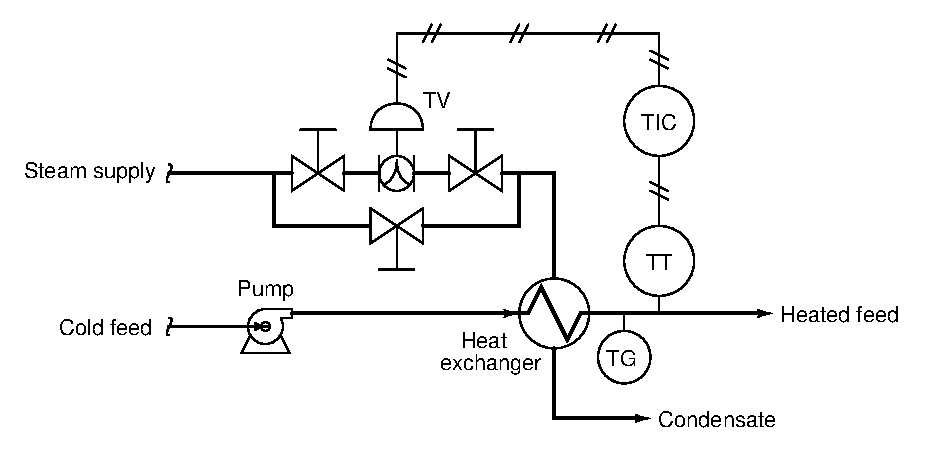
\includegraphics[width=15.5cm]{i00066x01.eps}$$

En rutinemessig vedlikeholdsoppgave du er tildelt er a ``stroke-teste'' reguleringsventilen for a verifisere at dens slag ikke er hindret eller at kalibreringen ikke er for langt ute av posisjon.  Det eneste problemet er at dette ma gjores mens prosessen er ``live'' (mateflyt som varmes), og den pneumatiske regulatoren har ingen manuell modus.

\vskip 10pt

Skisser en plan som lar deg stroke-teste denne reguleringsventilen med minimal avbrudd i prosessen.  Punkter som skal adresseres inkluderer:

\begin{itemize}
\item{} Hvordan holde matetemperaturen pa setpunkt mens ventilen strokes
\vskip 5pt
\item{} Hvordan stroke ventilen fra 0\% til 100\% av omradet uten manuell modus i regulatoren
\end{itemize}

\vfil

\underbar{file i00066}
\eject
%(END_QUESTION)





%(BEGIN_ANSWER)

Dette er et vurdert sporsmal -- ingen svar eller hint gis!

%(END_ANSWER)





%(BEGIN_NOTES)

Pa en eller annen mate ma vi finne en mate a bevege reguleringsventilen gjennom hele slaglengden uten a pavirke dampstromningen gjennom varmeveksleren.  Heldigvis har vi blokk- og bypassventiler installert for a isolere reguleringsventilen fra prosessflyten.  A lukke blokkventilene vil hindre stromning gjennom reguleringsventilen, mens apning av bypassventilen vil gi en alternativ vei rundt reguleringsventilen for dampen slik at varmeveksleren fortsatt far en tilforsel av termisk energi for a holde temperaturen pa setpunkt (vist av temperaturmaleren TG).  A lukke blokkventilene og apne bypassventilen er en prosedyre som best gjor en stegvis i stedet for alt pa en gang, for a unnga a utsette systemet for termisk sjokk (f.eks. lukk en blokkventil litt, apn deretter bypassventilen).  Hvis det finnes en mengdemaler et sted langs damptilforselslinjen, vil dennes indikasjon vare til stor hjelp mens vi manuelt lukker blokkventilene og apner bypassventilen, og lar oss vite om dampstromningen har avviket mye fra den opprinnelige verdien.  Selvfolgelig vil temperaturmaleren ogsa fortelle oss det, men dens respons vil vare mye tregere og derfor vanskeligere a kontrollere etter.

\vskip 10pt

Etter at reguleringsventilen er fullstendig blokkert og bypasset, kan vi bruke en handpumpe (eller en presisjonsregulator koblet til instrumentluft) for a gi ``stroking''-signalet til ventilen mens regulatorens utgangsror er frakoblet ventilen.

%INDEX% Final Control Elements, valve: performing maintenance on live system

%(END_NOTES)


